\section{Decomposition of Labour-Supply Change}

\subsection{The model of continuous change: an overview}

To measure the isolated effect of demographic ageing on aggregate labour supply, this article uses the continuous-change model \citep{horiuchiDecompositionMethodBased2008}. This model decomposes the difference between two summary measures generated by the same process into several components, each representing the contribution of an underlying factor. The process is defined as a function \(f\), which takes the values of the factors as arguments and returns a summary measure. A technical summary of the method is provided in the annex.

\vspace{0.7em}\par
For each pair of consecutive years between 2005 and 2025, the decomposition allocates the change in aggregate labour supply using a nested three-level structure. The first level separates contributions by birthplace status, distinguishing Spanish and foreign-born populations. Within each birthplace group, the contribution is divided into four components: total population growth (\textit{tpop}), age structure (\textit{stx}), labour-market participation or activity rates (\textit{wpx}), and hours worked (\textit{whx}). Finally, within each component, the contribution is split across age groups. Each contribution piece therefore represents the change in labour hours attributable to a specific age group within a specific component and birthplace group.


\vspace{0.7em}\par
A potential concern with the continuous-change model (CCM) is that it assumes smooth transitions between states, whereas Spain’s labour market was marked by sharp regime changes during the Great Recession, the migration reversal after 2008, and the COVID--19 shock. Although these episodes clearly violate economic smoothness, the CCM remains appropriate for the present analysis for two main reasons.

\vspace{0.7em}\par
First, the CCM does not impose continuity in economic outcomes or behavioural adjustments; continuity applies only to the accounting path used to allocate observed changes across factors. Abrupt movements in employment, migration, or participation are therefore fully captured in the underlying data, and the decomposition integrates these discrete changes mechanically over time without smoothing or averaging away shocks. Moreover, the decomposition is implemented on a year-by-year basis and reported over sub-periods that closely correspond to major regime shifts (2005--2009, 2010--2014, 2015--2019, and 2020--2025). This effectively yields a piecewise application of the CCM, allowing crisis-period dynamics to be identified explicitly rather than diluted within longer trends.

\vspace{0.7em}\par
Second, a central property of the CCM is its additivity, which holds by construction even in the presence of structural breaks. As illustrated in Table \ref{tab:effectMat}: the sum of the contribution pieces across all consecutive-year decompositions equals the corresponding contribution obtained from a decomposition between the first and last years. In addition, the sum of all contribution pieces equals the observed difference in aggregate labour supply between the two years, before decomposition. During crisis periods, this additivity should be interpreted strictly as an accounting identity rather than as evidence of economically smooth adjustment mechanisms. The CCM is thus used as a descriptive tool to allocate observed changes in labour supply across demographic and behavioural components, not as a model of adjustment dynamics.

\vspace{0.7em}\par
Taken together, these features make the CCM a transparent and internally consistent framework for assessing how ageing, migration, participation, and hours worked contribute to labour-supply change, even in periods marked by pronounced labour-market disruptions.






\subsection{Demographic and Behavioural Contributions}

Table \ref{tab:effectMat} shows the contribution of each component by birthplace and period, expressed in millions of full-time equivalent (FTE) workers, where one FTE corresponds to 2,000 annual hours worked. Positive values indicate contributions that increase aggregate labour supply; negative values indicate contributions that reduce it. The table shows that Spain's aggregate labour supply increased by \(2.18\) million FTE workers between 2005 and 2025, but this net gain hides a strong contrast by birthplace. The foreign-born contribution was strongly positive, adding \(3.04\) million FTE workers, while the Spanish contribution was negative, reducing labour supply by \(0.86\) million FTE workers.


\begin{table}[H]%
  \caption{Decomposition of changes in aggregate labour supply by birthplace, component, and period, Spain.}

  %\source{Author's calculations}
  \label{tab:effectMat}%
  \begin{center}
    \input{../resrc/effectMat.tex}%
    \caption*{\small Note: Values are expressed in millions of full-time equivalent (FTE) workers.}
  \end{center}
\end{table}%



\vspace{0.7em}\par
The main negative force is age structure among Spanish. For Spanish, the age-structure component reduced labour supply by \(2.55\) million FTE workers over 2005--2025. This confirms that population ageing among Spanish exerted a large downward pressure. However, this was more than offset by higher Spanish activity rates, which added \(2.82\) million FTE workers, while Spanish population size added \(0.46\) million. Declining hours worked reduced Spanish labour supply by another \(1.60\) million. For foreigners, the main positive contribution comes from population size, which added \(3.56\) million FTE workers. By contrast, foreign age structure slightly reduced labour supply by \(0.14\) million, foreign activity rates contributed almost nothing over the full period, at \(0.01\) million, and foreign hours worked reduced labour supply by \(0.39\) million. This means immigration's contribution came mainly through foreign population growth, not through higher participation or longer hours.

\vspace{0.7em}\par
Across periods, the strongest positive aggregate change occurred in 2005--2009, at \(1.64\) million FTE workers, and 2020--2025, at \(1.17\) million FTE workers. The period 2010--2014 was negative, at \(-0.57\) million, reflecting crisis-era weakness, while 2015--2019 was also slightly negative, at \(-0.05\) million. Overall, foreign population growth offset much of the negative age-structure effect among Spanish, but declining hours worked remained a drag across both groups. The relative contribution of these components across the major age groups is summarized in Figure \ref{fig:labDecomp}.


\subsection{Contribution of Ageing and Labour Components}

Figure \ref{fig:labDecomp} contains three panels distinguishing Spanish, foreign-born, and combined contributions to total labour-supply change between 2005 and 2025. Within each panel, the four bars correspond to the decomposition components: total population growth (\textit{tpop}), age structure (\textit{stx}), activity or participation rates (\textit{wpx}), and hours worked (\textit{whx}). The age-group contribution pieces are grouped into three major age groups: young workers aged 16--34, adults aged 35--54, and older workers aged 55 and over. These age-group contributions are divided by the total change in aggregate labour supply, so each bar represents the percentage of total change attributable to a specific age group within a specific component and birthplace group. For the Spanish and foreign panels, the age-group contributions across all components sum jointly to 100\%, because these two panels add up to the total change in aggregate labour supply. In contrast, the combined panel aggregates Spanish and foreign contributions first; within this panel, the age-group contributions across all components also sum to 100\%. Positive values indicate contribution pieces that increased labour supply, while negative values indicate contribution pieces that reduced it.

\begin{figure}[H]%
  \caption{Contribution of demographic and behavioural factors expressed as a percentage of the total variation in aggregate labour supply, Spain 2005--2025}%
  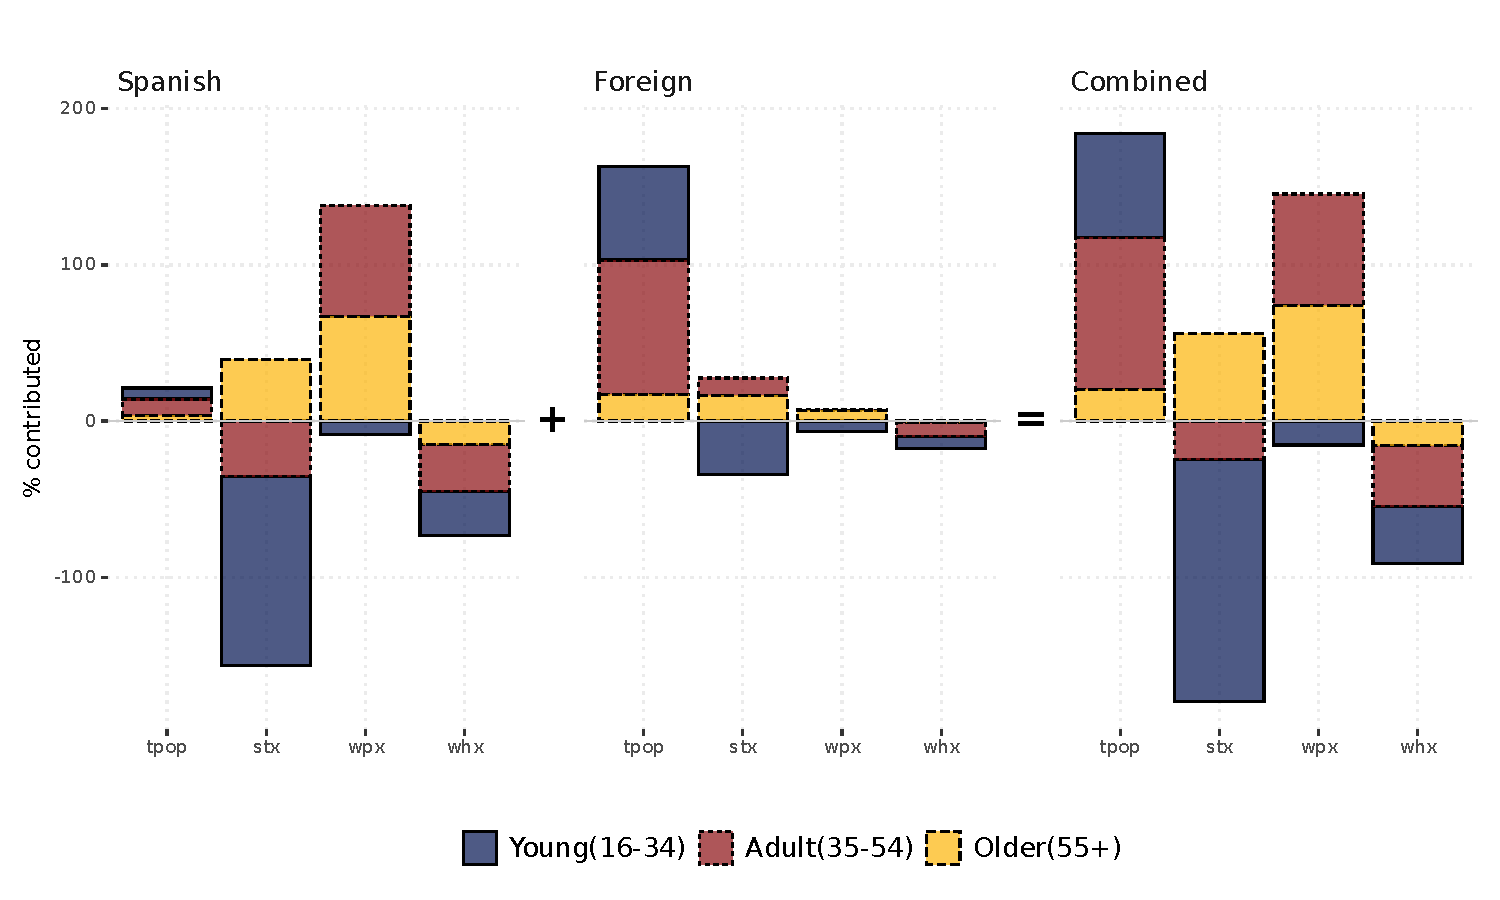
\includegraphics[width=1\textwidth]{../resrc/labDecomp.pdf}%
  \label{fig:labDecomp}%
\end{figure}%




By far, the largest negative contributions come from age-structure changes among younger and prime-age groups. The strongest drag is the age-structure effect for young Spanish aged 16--34, which contributes \(-120.8\%\) of the total change, followed by the age-structure effect for Spanish adults aged 35--54, at \(-35.6\%\). The age-structure effect for young foreigners is also negative, at \(-34.2\%\). In contrast, the largest positive contributions come from foreign population growth among adults aged 35--54, which contributes \(86.3\%\), and from higher activity rates among Spanish adults and older workers, contributing \(70.9\%\) and \(67.1\%\), respectively. Thus, the main offset to demographic ageing within the Spanish-born population comes from foreign prime-age population growth and stronger labour-market attachment among Spanish adults and older workers.




